\begin{center}
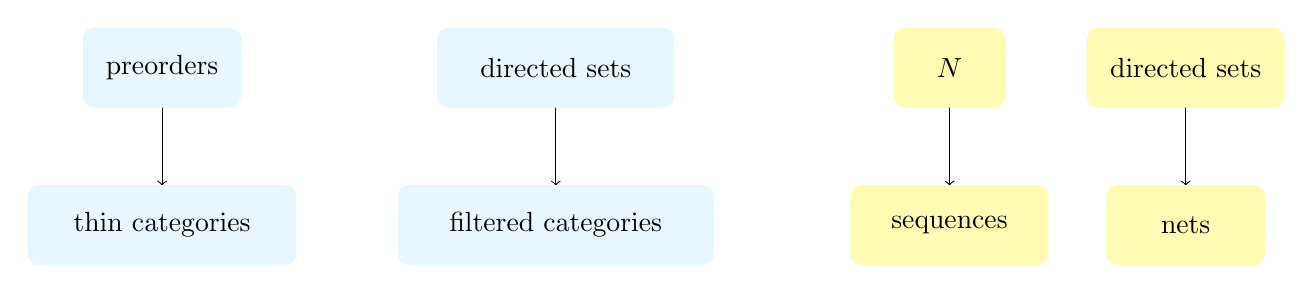
\begin{tikzpicture}
\begin{scope}[xshift = -3cm]
\draw[->] (0,-0.5)--(0, -1.5);
\draw[->] (5,-0.5)--(5, -1.5);
\filldraw[rounded corners, ProcessBlue!10]
(-1,-0.5) rectangle (1, 0.5);
\node at (0,0) {preorders};

\begin{scope}[xshift = 5cm]
\filldraw[rounded corners, ProcessBlue!10]
(-1.5,-0.5) rectangle (1.5, 0.5);
\node at (0,0) {directed sets};
\end{scope}

\begin{scope}[yshift = -2cm]
\filldraw[rounded corners, ProcessBlue!10]
(-1.7,-0.5) rectangle (1.7, 0.5);
\node at (0,0) {thin categories};
\end{scope}

\begin{scope}[xshift = 5cm, yshift=-2cm]
\filldraw[rounded corners, ProcessBlue!10]
(-2,-0.5) rectangle (2, 0.5);
\node at (0,0) {filtered categories};
\end{scope}
\end{scope}

\begin{scope}[xshift = 7cm]
\draw[->] (0,-0.5)--(0, -1.5);
\draw[->] (3,-0.5)--(3, -1.5);
\filldraw[rounded corners, yellow!30]
(-0.7,-0.5) rectangle (0.7, 0.5);
\node at (0,0) {$\mathbb{N}$};

\begin{scope}[xshift = 3cm]
\filldraw[rounded corners, yellow!30]
(-1.25,-0.5) rectangle (1.25, 0.5);
\node at (0,0) {directed sets};
\end{scope}

\begin{scope}[yshift = -2cm]
\filldraw[rounded corners, yellow!30]
(-1.25,-0.5) rectangle (1.25, 0.5);
\node at (0,0) {sequences};
\end{scope}

\begin{scope}[xshift = 3cm, yshift=-2cm]
\filldraw[rounded corners, yellow!30]
(-1,-0.5) rectangle (1, 0.5);
\node at (0,0) {nets};
\end{scope}
\end{scope}
\end{tikzpicture}

\emph{On the left, we see that thin and filtered categories are the categorification of 
concepts which we will use to take limits over. On the right, we have topology concepts 
of sequences and nets, which are limits taken over different sets. }
\end{center}